% Created by tikzDevice version 0.12 on 2019-01-03 18:24:32
% !TEX encoding = UTF-8 Unicode
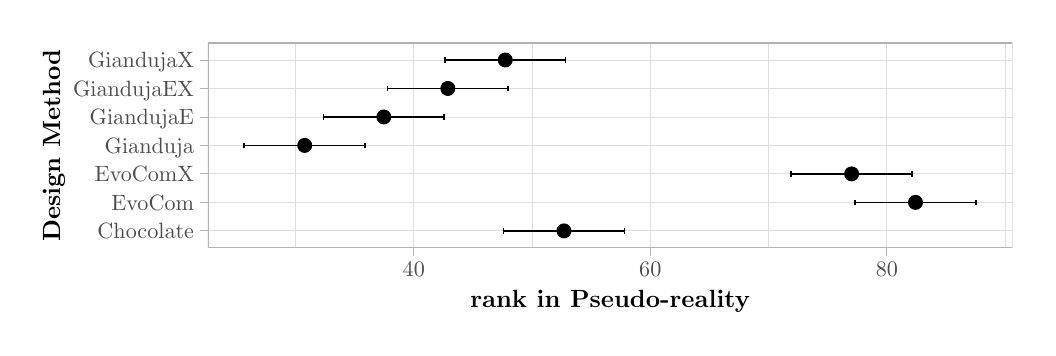
\begin{tikzpicture}[x=1pt,y=1pt]
\definecolor{fillColor}{RGB}{255,255,255}
\path[use as bounding box,fill=fillColor,fill opacity=0.00] (0,0) rectangle (361.35,108.41);
\begin{scope}
\path[clip] (  0.00,  0.00) rectangle (361.35,108.40);
\definecolor{drawColor}{RGB}{255,255,255}
\definecolor{fillColor}{RGB}{255,255,255}

\path[draw=drawColor,line width= 0.6pt,line join=round,line cap=round,fill=fillColor] (  0.00,  0.00) rectangle (361.35,108.40);
\end{scope}
\begin{scope}
\path[clip] ( 65.07, 28.81) rectangle (355.85,102.90);
\definecolor{fillColor}{RGB}{255,255,255}

\path[fill=fillColor] ( 65.07, 28.81) rectangle (355.85,102.90);
\definecolor{drawColor}{gray}{0.87}

\path[draw=drawColor,line width= 0.1pt,line join=round] ( 96.78, 28.81) --
	( 96.78,102.90);

\path[draw=drawColor,line width= 0.1pt,line join=round] (182.25, 28.81) --
	(182.25,102.90);

\path[draw=drawColor,line width= 0.1pt,line join=round] (267.72, 28.81) --
	(267.72,102.90);

\path[draw=drawColor,line width= 0.1pt,line join=round] (353.19, 28.81) --
	(353.19,102.90);

\path[draw=drawColor,line width= 0.3pt,line join=round] ( 65.07, 34.98) --
	(355.85, 34.98);

\path[draw=drawColor,line width= 0.3pt,line join=round] ( 65.07, 45.27) --
	(355.85, 45.27);

\path[draw=drawColor,line width= 0.3pt,line join=round] ( 65.07, 55.57) --
	(355.85, 55.57);

\path[draw=drawColor,line width= 0.3pt,line join=round] ( 65.07, 65.86) --
	(355.85, 65.86);

\path[draw=drawColor,line width= 0.3pt,line join=round] ( 65.07, 76.15) --
	(355.85, 76.15);

\path[draw=drawColor,line width= 0.3pt,line join=round] ( 65.07, 86.44) --
	(355.85, 86.44);

\path[draw=drawColor,line width= 0.3pt,line join=round] ( 65.07, 96.73) --
	(355.85, 96.73);

\path[draw=drawColor,line width= 0.3pt,line join=round] (139.52, 28.81) --
	(139.52,102.90);

\path[draw=drawColor,line width= 0.3pt,line join=round] (224.99, 28.81) --
	(224.99,102.90);

\path[draw=drawColor,line width= 0.3pt,line join=round] (310.46, 28.81) --
	(310.46,102.90);
\definecolor{drawColor}{RGB}{0,0,0}
\definecolor{fillColor}{RGB}{0,0,0}

\path[draw=drawColor,line width= 0.4pt,line join=round,line cap=round,fill=fillColor] (193.79, 34.98) circle (  2.50);

\path[draw=drawColor,line width= 0.4pt,line join=round,line cap=round,fill=fillColor] (320.81, 45.27) circle (  2.50);

\path[draw=drawColor,line width= 0.4pt,line join=round,line cap=round,fill=fillColor] (297.73, 55.57) circle (  2.50);

\path[draw=drawColor,line width= 0.4pt,line join=round,line cap=round,fill=fillColor] (100.11, 65.86) circle (  2.50);

\path[draw=drawColor,line width= 0.4pt,line join=round,line cap=round,fill=fillColor] (128.69, 76.15) circle (  2.50);

\path[draw=drawColor,line width= 0.4pt,line join=round,line cap=round,fill=fillColor] (151.82, 86.44) circle (  2.50);

\path[draw=drawColor,line width= 0.4pt,line join=round,line cap=round,fill=fillColor] (172.57, 96.73) circle (  2.50);

\path[draw=drawColor,line width= 0.6pt,line join=round] (215.62, 33.95) --
	(215.62, 36.01);

\path[draw=drawColor,line width= 0.6pt,line join=round] (215.62, 34.98) --
	(171.97, 34.98);

\path[draw=drawColor,line width= 0.6pt,line join=round] (171.97, 33.95) --
	(171.97, 36.01);

\path[draw=drawColor,line width= 0.6pt,line join=round] (342.63, 44.25) --
	(342.63, 46.30);

\path[draw=drawColor,line width= 0.6pt,line join=round] (342.63, 45.27) --
	(298.98, 45.27);

\path[draw=drawColor,line width= 0.6pt,line join=round] (298.98, 44.25) --
	(298.98, 46.30);

\path[draw=drawColor,line width= 0.6pt,line join=round] (319.56, 54.54) --
	(319.56, 56.59);

\path[draw=drawColor,line width= 0.6pt,line join=round] (319.56, 55.57) --
	(275.91, 55.57);

\path[draw=drawColor,line width= 0.6pt,line join=round] (275.91, 54.54) --
	(275.91, 56.59);

\path[draw=drawColor,line width= 0.6pt,line join=round] (121.93, 64.83) --
	(121.93, 66.89);

\path[draw=drawColor,line width= 0.6pt,line join=round] (121.93, 65.86) --
	( 78.28, 65.86);

\path[draw=drawColor,line width= 0.6pt,line join=round] ( 78.28, 64.83) --
	( 78.28, 66.89);

\path[draw=drawColor,line width= 0.6pt,line join=round] (150.52, 75.12) --
	(150.52, 77.18);

\path[draw=drawColor,line width= 0.6pt,line join=round] (150.52, 76.15) --
	(106.87, 76.15);

\path[draw=drawColor,line width= 0.6pt,line join=round] (106.87, 75.12) --
	(106.87, 77.18);

\path[draw=drawColor,line width= 0.6pt,line join=round] (173.64, 85.41) --
	(173.64, 87.47);

\path[draw=drawColor,line width= 0.6pt,line join=round] (173.64, 86.44) --
	(129.99, 86.44);

\path[draw=drawColor,line width= 0.6pt,line join=round] (129.99, 85.41) --
	(129.99, 87.47);

\path[draw=drawColor,line width= 0.6pt,line join=round] (194.39, 95.70) --
	(194.39, 97.76);

\path[draw=drawColor,line width= 0.6pt,line join=round] (194.39, 96.73) --
	(150.74, 96.73);

\path[draw=drawColor,line width= 0.6pt,line join=round] (150.74, 95.70) --
	(150.74, 97.76);
\definecolor{drawColor}{gray}{0.70}

\path[draw=drawColor,line width= 0.6pt,line join=round,line cap=round] ( 65.07, 28.81) rectangle (355.85,102.90);
\end{scope}
\begin{scope}
\path[clip] (  0.00,  0.00) rectangle (361.35,108.41);
\definecolor{drawColor}{gray}{0.30}

\node[text=drawColor,anchor=base east,inner sep=0pt, outer sep=0pt, scale=  0.80] at ( 60.12, 32.23) {Chocolate};

\node[text=drawColor,anchor=base east,inner sep=0pt, outer sep=0pt, scale=  0.80] at ( 60.12, 42.52) {EvoCom};

\node[text=drawColor,anchor=base east,inner sep=0pt, outer sep=0pt, scale=  0.80] at ( 60.12, 52.81) {EvoComX};

\node[text=drawColor,anchor=base east,inner sep=0pt, outer sep=0pt, scale=  0.80] at ( 60.12, 63.10) {Gianduja};

\node[text=drawColor,anchor=base east,inner sep=0pt, outer sep=0pt, scale=  0.80] at ( 60.12, 73.39) {GiandujaE};

\node[text=drawColor,anchor=base east,inner sep=0pt, outer sep=0pt, scale=  0.80] at ( 60.12, 83.68) {GiandujaEX};

\node[text=drawColor,anchor=base east,inner sep=0pt, outer sep=0pt, scale=  0.80] at ( 60.12, 93.98) {GiandujaX};
\end{scope}
\begin{scope}
\path[clip] (  0.00,  0.00) rectangle (361.35,108.41);
\definecolor{drawColor}{gray}{0.70}

\path[draw=drawColor,line width= 0.3pt,line join=round] ( 62.32, 34.98) --
	( 65.07, 34.98);

\path[draw=drawColor,line width= 0.3pt,line join=round] ( 62.32, 45.27) --
	( 65.07, 45.27);

\path[draw=drawColor,line width= 0.3pt,line join=round] ( 62.32, 55.57) --
	( 65.07, 55.57);

\path[draw=drawColor,line width= 0.3pt,line join=round] ( 62.32, 65.86) --
	( 65.07, 65.86);

\path[draw=drawColor,line width= 0.3pt,line join=round] ( 62.32, 76.15) --
	( 65.07, 76.15);

\path[draw=drawColor,line width= 0.3pt,line join=round] ( 62.32, 86.44) --
	( 65.07, 86.44);

\path[draw=drawColor,line width= 0.3pt,line join=round] ( 62.32, 96.73) --
	( 65.07, 96.73);
\end{scope}
\begin{scope}
\path[clip] (  0.00,  0.00) rectangle (361.35,108.41);
\definecolor{drawColor}{gray}{0.70}

\path[draw=drawColor,line width= 0.3pt,line join=round] (139.52, 26.06) --
	(139.52, 28.81);

\path[draw=drawColor,line width= 0.3pt,line join=round] (224.99, 26.06) --
	(224.99, 28.81);

\path[draw=drawColor,line width= 0.3pt,line join=round] (310.46, 26.06) --
	(310.46, 28.81);
\end{scope}
\begin{scope}
\path[clip] (  0.00,  0.00) rectangle (361.35,108.41);
\definecolor{drawColor}{gray}{0.30}

\node[text=drawColor,anchor=base,inner sep=0pt, outer sep=0pt, scale=  0.80] at (139.52, 18.35) {40};

\node[text=drawColor,anchor=base,inner sep=0pt, outer sep=0pt, scale=  0.80] at (224.99, 18.35) {60};

\node[text=drawColor,anchor=base,inner sep=0pt, outer sep=0pt, scale=  0.80] at (310.46, 18.35) {80};
\end{scope}
\begin{scope}
\path[clip] (  0.00,  0.00) rectangle (361.35,108.41);
\definecolor{drawColor}{RGB}{0,0,0}

\node[text=drawColor,anchor=base,inner sep=0pt, outer sep=0pt, scale=  0.90] at (210.46,  7.44) {\bfseries rank in Pseudo-reality};
\end{scope}
\begin{scope}
\path[clip] (  0.00,  0.00) rectangle (361.35,108.41);
\definecolor{drawColor}{RGB}{0,0,0}

\node[text=drawColor,rotate= 90.00,anchor=base,inner sep=0pt, outer sep=0pt, scale=  0.90] at ( 11.71, 65.86) {\bfseries Design Method};
\end{scope}
\end{tikzpicture}
